\documentclass[../main.tex]{subfiles}

\begin{document}
\subsection{Integrales ``Complejas''}
\classdate{2026-04-07}

\begin{definition}
    Sean \(I \subset \mathbb{R}\) un intervalo, \(f \colon I \subseteq \mathbb{R} \to
    \mathbb{C}\) y \(\bigl[a,b\bigr] \subseteq I\). Definimos

    \begin{equation}
        \int_{a}^{b}\odif[sep-end=\medspace]{t} f(t) =
        \int_{a}^{b}\odif[sep-end=\medspace]{t}
        \Re(f(t)) + i \int_{a}^{b}\odif[sep-end=\medspace]{t} \Im(f(t)).
    \end{equation}
\end{definition}
\begin{property}
    Sean \(f,g \colon I \subseteq \mathbb{R} \to \mathbb{C}\) funciones continuas en
    \(I\) y \(\bigl[a,b\bigr]\in I\). Entonces

    \begin{enumerate}
        \item \(\Re \Bigl(\int_{a}^{b}\odif[sep-end=\medspace]{t} f(t)\Bigr) =
                \int_{a}^{b}\odif[sep-end=\medspace]{t} \Re(f(t)),\quad
                \Im \Bigl(\int_{a}^{b}\odif[sep-end=\medspace]{t} f(t)\Bigr) =
            \int_{a}^{b}\odif[sep-end=\medspace]{t} \Im(f(t)).\)
        \item Si \(\lambda \in \mathbb{C}\),
            \begin{equation}
                \int_{a}^{b}\odif[sep-end=\medspace]{t} (f + \lambda g)(t) =
                \int_{a}^{b}\odif[sep-end=\medspace]{r} f(t) + \lambda
                \int_{a}^{b}\odif[sep-end=\medspace]{t} g(t)
            \end{equation}
            .
        \item (Desigualdad del triángulo)
            \begin{equation}
                \abs`\Bigg{\int_{a}^{b}\odif[sep-end=\medspace]{t} f(t)} \leq
                \int_{a}^{b}\odif[sep-end=\medspace]{t} \abs{f(t)}
            \end{equation}
    \end{enumerate}
\end{property}
\begin{proof}
    \begin{enumerate}[start=3]
        \item Sea \(\lambda = \int_{a}^{b}\odif[sep-end=\medspace]{t} f(t)\). Si
            \(\lambda = 0\), entonces

            \begin{equation}
                \abs`\Bigg{\int_{a}^{b}\odif[sep-end=\medspace]{t} f(t)} = \abs{0} \leq
                \int_{a}^{b}\odif[sep-end=\medspace]{t} \abs{f(t)},
            \end{equation}

            pues \(\abs{f(t)} \geq 0\;\forall t\in I\).

            Supongamos \(\lambda \neq 0\). Entonces, \(\lambda =
            \abs{\lambda}\mathrm{e}^{i\theta}\), donde el argumento principal
            es \(\theta =
            \arg(\lambda)\in (-\pi, \pi]\). Despejando \(\abs{\lambda} = \lambda
            \mathrm{e}^{-i\theta}\),

            \begin{align}
                \abs`\Bigg{\int_{a}^{b}\odif[sep-end=\medspace]{t} f(t)} =
                \abs{\lambda} & =
                \Re(\abs{\lambda})  = \Re \bigl(\lambda
                \mathrm{e}^{-i\theta}\bigr),\nonumber
                \\
                & = \Re \Bigl(\int_{a}^{b}\odif[sep-end=\medspace]{t}
                \mathrm{e}^{-i\theta}f(t)\Bigr) =
                \int_{a}^{b}\odif[sep-end=\medspace]{t}
                \Re(\mathrm{e}^{-i\theta}) ,\nonumber
                \\
                & \leq \int_{a}^{b}\odif[sep-end=\medspace]{t}
                \abs{\mathrm{e}^{-i\theta}f(t)},\nonumber
                \\\shortintertext{Por monotonía\footnote{Comportamiento completamente
                decreciente o completamente decreciente.} de la integral real}
                & = \int_{a}^{b}\odif[sep-end=\medspace]{t}
                \underbrace{\abs{\mathrm{e}^{-i\theta}}}_{=
                1}\abs{f(t)},\nonumber
                \\
                & = \int_{a}^{b}\odif[sep-end=\medspace]{t} \abs{f(t)}.
            \end{align}
    \end{enumerate}
\end{proof}

\begin{definition}
    Sea \(\gamma \colon  \bigl[a,b\bigr] \subseteq \mathbb{R} \to \mathbb{C}\). Decimos
    que \(\gamma\) es una parametrización suave por pedazos si existe una partición \(P
    = \{a = t_{0} < \cdots < t_{k} = b\}\) de \(\bigl[a,b\bigr]\) tal que
    \(\eval{\gamma}{\bigl[t_{i-1}, t_{i}\bigr]}\) es de clase \(C^{1}\)
    \(\forall i \in \{1,
    \dots k\}\). A la imagen \(\Gamma \coloneqq \gamma([a,b])\) se le conoce como curva
    suave por pedazos parametrizada por \(\gamma\). A \(\gamma(a)\) se le conoce como el
    punto inicial de la curva y a \(\gamma(b)\) como el punto final de \(\Gamma\). Si
    \(\gamma(a) = \gamma(b)\), decimos que \(\Gamma\) es una curva cerrada.

    \begin{figure}[htb]
        \centering
        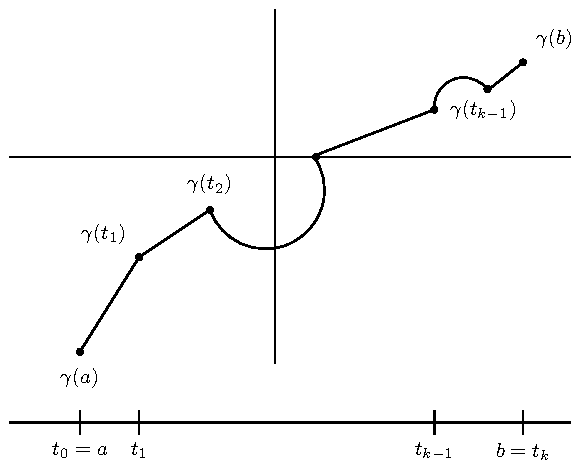
\includegraphics[width=0.5\linewidth]{../figs/build/suave-a-pedazos.pdf}
    \end{figure}
\end{definition}

\begin{definition}
    Sean \(\gamma \colon [a,b] \to \mathbb{C}\) y \(\delta \colon [c,d]  \to
    \mathbb{C}\)
    curvas suaves por pedazos tales que \(\gamma(b) = \delta(c)\). Definimos la
    concatenación de \(\gamma\) y \(\delta\) denotada por \(\gamma + \delta
        (\gamma \star
    \delta)\), como

    \begin{equation}
        \gamma + \delta \coloneqq \bigl[a, b + (d - c)\bigr] \to \mathbb{C}
    \end{equation}

    dada por

    \begin{equation}
        (\gamma + \delta)(t) =
        \begin{dcases}
            \gamma(t)         & \text{si}\; t \in [a,b],            \\
            \delta(c + t - b) & \text{si}\; t \in [b, b + (d - c)].
        \end{dcases}
    \end{equation}
\end{definition}

También definimos \(-\gamma \colon [a,b] \to \mathbb{C}\) que ``recorre \(\Gamma =
\gamma([a,b])\) en sentido opuesto'' como

\begin{equation}
    (-\gamma)(t) = \gamma(a + b - t).
\end{equation}

\begin{definition}
    Sean \(f \colon \Omega \subseteq \mathbb{C} \to \mathbb{C}\) continua y \(\gamma
    \colon [a, b] \to \mathbb{C}\) una curva suave por pedazos tal que \(\gamma([a,b])
    \subseteq \Omega\).

    \begin{enumerate}
        \item Definimos la integral de línea de \(f\) sobre \(\gamma\) dada por longitud
            de arco como

            \begin{equation}
                \int_{\gamma} \abs{\odif[sep-end=\medspace]{z}} f(z) \coloneqq
                \int_{a}^{b}\odif[sep-end=\medspace]{t} \abs{\gamma^{\prime}(t)}
                f(\gamma(t)).
            \end{equation}
        \item Definimos la integral de línea de \(f\) sobre \(\gamma\) como

            \begin{equation}
                \int_{\gamma}\odif[sep-end=\medspace]{z} f(z) \coloneqq
                \int_{a}^{b}\odif[sep-end=\medspace]{t} f(\gamma(t))\gamma^{\prime}(t).
            \end{equation}
    \end{enumerate}
\end{definition}
\end{document}
